\chapter{Revisão Sistemática de Literatura}
\label{chapter:revisao}

Este capítulo apresenta todas as informações relevantes para a condução da Revisão Sistemática de Literatura conduzida neste projeto de pesquisa.

\section{Informações Gerais}

A presente revisão sistemática é entitulada de ``Uma Revisão Sistemática sobre Aprendizado e Sugestão Automatizada de Modificações de Código-Fonte utilizando o Histórico de Versão'', a qual tem como intuito identificar as principais técnicas e abordagens utilizadas no processo de aprendizagem de modificações e como classificar tais melhorias/degradações de código-fonte, com base no impacto gerado em métricas de qualidade, através da análise histórico de versão em repositórios de software.

O grupo de pesquisadores envolvidos é composto pelos seguintes membros:

\begin{itemize}
\item \textbf{Nome:} Leandro Ungari Cayres\\
	  \textbf{E-mail:} leandro.ungari@unesp.br\\
	  \textbf{Currículo Lattes:} http://lattes.cnpq.br/5996829502147029\\
\item \textbf{Nome:} Bruno Santos de Lima\\
	  \textbf{E-mail:} bruno.s.lima@unesp.br\\
	  \textbf{Currículo Lattes:} http://lattes.cnpq.br/2119168921461476\\
\item \textbf{Nome:} Rogério Eduardo Garcia\\
	  \textbf{E-mail:} rogerio.garcia@unesp.br\\
	  \textbf{Currículo Lattes:} http://lattes.cnpq.br/8031012573259361\\

\end{itemize}

A condução dessa revisão tem como intuito formar uma base de conhecimento que colabore com a condução dos estudos especiais, assim como base para o restante do curso de Mestrado.

\section{Questões de Pesquisa}
\label{label:questoes-pesquisa}

De modo a identificar os pontos de investigação dentro da revisão sistemática, foram elaboradas as seguintes questões de pesquisa:

\begin{itemize}
\item QP1: Como modificações são detectadas entre versões de código-fonte?
\item QP2: Como são aplicadas modificações de código-fonte?
\item QP3: Como identificar padrões comuns entre modificações de código-fonte?
\item QP4: Como modificações de código-fonte em geral podem ser classificadas entre melhorias e degradações?
%\item QP4: Como detectar se a moficação pode modificar a funcionalidade implementada?
\item QP5: Como a sugestão de modificações é feita ao usuário?

\end{itemize}

A elaboração das questões de pesquisa foi realizada com base nos critérios PICO apresentados na Tabela~\ref{table:pico}.

\begin{table}[h]
\centering
\label{table:pico}
\begin{tabular}{L{3cm}|L{10cm}}
\hline
População & Técnicas e abordagens que analisam modificações em repositórios de software. \\
\hline
Intervenção & A utilização do histórico do código-fonte na realização de melhorias do código-fonte.\\
\hline
Comparação & Não se aplica.\\
\hline
Resultados & Visão geral dos estudos quanto ao uso do histórico de modificações para melhoria do software, quanto aos métodos e tecnologias utilizadas de modo que permita a realização do propósito do estudo.\\
\hline

\end{tabular}
\caption{Critérios PICO.}
\end{table}


\section{Identificação de Estudos}

\subsection{\emph{String} de Busca}

O primeiro passo para a condução da busca consiste na determinação de termos relevantes para a composição da~\emph{string} de busca. A Tabela~\ref{table:palavras-chave} apresenta as palavras-chave definidas:

\begin{table}[h]
\centering
\label{table:palavras-chave}
\begin{tabular}{L{3cm}|L{10cm}}
\hline
Palavras-chave & ~\emph{"code transformation", "code change", "code edit", "version", improvement", "degradation", "learning", "code history", "code pattern"}. \\
\hline
\end{tabular}
\caption{Palavras-chave da revisão sistemática.}
\end{table}

A partir desse conjunto de palavras-chave foi definida a seguinte~\emph{string} de busca para a execução da busca:

\begin{center}
\emph{("code" OR "source code" OR "code pattern") AND\\ 
("edit" OR "change" OR "transformation") AND\\
(("learning") OR ("history" OR "version"))}
\end{center}

\subsection{Fontes de Busca}
As fontes de busca selecionadas para realizar a busca por estudos são conhecidas por serem as principais bases bibliográficas em Ciência da Computação~\citep{nakagawa2017revisao} e são fontes de buscas nas quais os pesquisadores envolvidos na elaboração da revisão sistemática têm acesso.

A Tabela~\ref{table:fontes-busca} apresenta as bases bibliográficas utilizadas:

\begin{table}[h]
\centering
\label{table:fontes-busca}
\begin{tabular}{L{4cm}|L{7cm}|L{3cm}}
\hline
\textbf{Fonte de Busca} & \textbf{Endereço Online} & \textbf{Tipo}\\
\hline
\emph{IEEE Xplore} & \url{ieeexplore.ieee.org} & Base Bibliográfica\\
\hline
\emph{ACM Digital Library} & \url{dl.acm.org} & Híbrida \\
\hline
\emph{Enginnering Village} & \url{http://www.engineeringvillage.com} & Motor de Busca \\
\hline
\emph{Science Direct} & \url{https://www.sciencedirect.com/} & Base Bibliográfica \\
\hline
\end{tabular}
\caption{Fontes de busca da revisão sistemática.}
\end{table}


\subsection{Estratégia de Busca}

As buscas foram realizadas de forma automatizada das bases bibliográficas, em que a~\emph{string} de busca foi aplicada aos campos de título, resumo e palavras-chave. 
Vale ressaltar que foram conduzidas buscas-piloto com o intuito de aprimorar a~\emph{string} de busca.

Também foi aplicada a estratégia~\emph{Snowballing Avante} em cada um dos artigos resultantes da busca automatizada, visando identificar novos estudos primários que possam ser relevantes para a Revisão Sistemática da literatura.

Todos os estudos selecionados estavam delimitados aoperíodo de 2012 a 2019. 
Adicionalmente, não foram realizadas consultas a especialistas, assim como buscas manuais.


\section{Seleção e Avaliação de Estudos}

O processo de seleção é dividido em duas etapas: Seleção inicial, na qual critérios de seleção são aplicados em todos os estudos identificados após a leitura de seu título e resumo, os estudos só serão excluídos se eles atenderem a pelo menos um critério de exclusão. Seleção final, segunda etapa, na qual os estudo selecionados na etapa anterior são analisados com maiores detalhes após sua leitura completa seguindo os critérios de seleção. Após isso, os estudos incluídos são avaliados com base nos critérios de qualidade~\citep{nakagawa2017revisao}. 

\subsection{Critérios de Avaliação}
A seguir estão listados os critérios de inclusão e exclusão, os quais serão utilizados no processo de seleção dos estudos obtidos da busca nos mecanismos de pesquisa.

\begin{itemize}
\item~\textbf{Critérios de Inclusão:}
\begin{enumerate}
\item O estudo apresenta análise do histórico de versões do código-fonte no contexto de modificações de código-fonte ou análise de qualidade de código.
\item O estudo apresenta técnicas, abordagens relativas a detecção de modificações no código-fonte. 
\item O estudo propõe ou relata algo relativo a aprendizado automatizado de modificações com análise direta do código-fonte.
\item O estudo relaciona-se ao aprendizado de padrões de modificação de código-fonte.
\item O estudo relaciona-se a mensuração da qualidade de código em modificações de código-fonte.
\item O estudo analisa o impacto de melhorias, defeitos na qualidade do código-fonte.
\item O estudo relata o uso de métricas para análise e classificação da qualidade do código-fonte.
\item O estudo apresenta alguma estratégia do sugestão de modificações.
\end{enumerate}
\item~\textbf{Critérios de Exclusão:}
\begin{enumerate}
\item O estudo não possui resumo.
\item O estudo somente está publicado como resumo ou pôster.
\item O estudo não está escrito em inglês.
\item O estudo é uma versão mais antiga do outro estudo já considerado.
\item O estudo não é um estudo primário.
\item Não foi possível ter acesso ao estudo.
\item O estudo foi publicado antes de 2012.
\item O estudo não apresenta análise do código-fonte direta, mas sim utiliza outras abordagens.
\item O estudo envolve modificações de código-fonte muito específicas de um dado contexto.
\item O estudo não é relacionado a área de Engenharia de Software.
\item O estudo não é relacionado a modificações de código-fonte.
\item O estudo é relacionado a modificações de código, mas não visa identificar, aprender ou analisar o impacto delas.
\item O estudo envolve modificações de código, porém é voltado para outras aplicações como visualização.
\end{enumerate}
\end{itemize}

\subsection{Estratégia de Seleção dos Estudos}

A estratégia para seleção de estudos está representada na Figura~\ref{image:selecao}. Todos os estudos resultantes da busca automatizada serão organizados visando remover estudos duplicados. 
Após a remoção de possíveis duplicações será executado em três etapas: 

\begin{itemize}
\item Eliminação de Duplicados
\item Seleção Inicial
\item Seleção Final
\end{itemize}

Toda etapa de seleção deve ser documentada utilizando planilhas eletrônicas, sendo uma planilha para cada etapa de seleção.

\begin{figure}[ht]
\label{image:selecao}
\centering
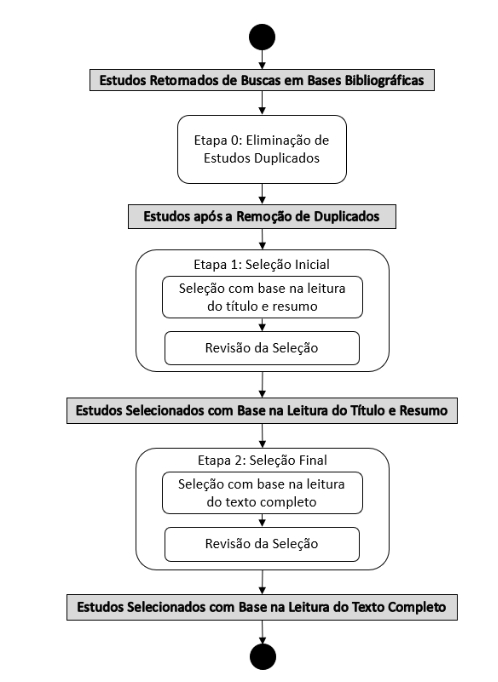
\includegraphics[width=.65\textwidth]{images/selecao.jpg}
\caption{Sequência de atividades da etapa de seleção -- adaptado de~\cite{nakagawa2017revisao}.}
\end{figure}

\subsection{Extração dos Dados}
As questões elaboradas para a extração dos dados correspondem a quatro níveis para avaliação da qualidade: (1) Filtro inicial;(2) Rigor; (3) Credibilidade e (4) Relevância. Cada estudo foi avaliado em cada questão no critério de "Não aceitável", "Fracamente aceitável" e "Aceitável", cuja pontuação respectivamente é 0, 0.5 e 1.

\begin{table}
\label{table:avaliacao}
\centering
\begin{tabular}{L{1cm} | L{12cm} }
\hline
ID & Questão \\
\hline
Q1 & O estudo é baseado em pesquisa ou somente relato de experiência?\\
\hline
Q2 & Os objetivos estão claramente definidos?\\
\hline
Q3 & O contexto em que o trabalho está inserido foi apresentado claramente?\\
\hline
Q4 & A abordagem/estratégia desenvolvida está descrita de forma clara?\\
\hline
Q5 &  Os pesquisadores analisaram as vantagens/desvantagens/limitações da abordagem/estratégia utilizada?\\
\hline
Q6 &  Qual a qualidade das questões de pesquisa elaboradas?\\
\hline
Q7 &  O estudo utiliza dados reais?\\
\hline
Q8 &  A obtenção e análise dos resultados foi descrita de forma clara?\\
\hline
Q9 &  Foi analisada a influência dos próprios pesquisadores nos resultados?\\
\hline
Q10 &  Há justificativa e discussão dos resultados?\\
\hline
Q11 &  Foram encontradas contribuições relevantes do estudo?\\
\hline
\end{tabular}
\caption{Questões de Avaliação de Qualidade -- adaptado de~\cite{marccal2016techniques}.}
\end{table}

A Tabela~\ref{table:qualidade} apresentada as categorias de classificação dos estudos:

\begin{table}[ht]
\label{table:qualidade}
\centering
\begin{tabular}{L{5cm} | L{5cm}}
\hline
Classificação & Pontuação\\
\hline
Muito Fraca Qualidade & 0 |- 3 \\
\hline
Fraca Qualidade & 3 |- 6,5 \\
\hline
Boa Qualidade & 6,5 |- 9 \\
\hline
Muito Boa Qualidade & 9 |-| 11 \\
\hline
\end{tabular}
\caption{Categorias de Classificação dos Estudos.}
\end{table}

Após a classificação dos estudos, somente os estudos que obtiveram "Boa Qualidade" e "Muito Boa Qualidade" foram selecionados. 
Por fim, de modo a extrair os dados dos estudos selecionados foi utilizado o conjunto de questões apresentado na Tabela~\ref{table:questoes-extracao}.

\begin{table}[ht]
\label{table:questoes-extracao}
\centering
\begin{tabular}{L{2cm} | L{10cm}}
\hline
Inf 1 & Identificador do Estudo\\
\hline
Inf 2 & Título \\
\hline
Inf 3 & Data de Extração\\
\hline
Inf 4 & Autores\\
\hline
Inf 5 & Ano\\
\hline
Inf 6 & Visão Geral do Estudo\\
\hline
Inf 7 & Contexto do Problema\\
\hline
Inf 8 & Objectivo do Estudo\\
\hline
Inf 9 & Estratégia da Abordagem/Técnica\\
\hline
Inf 10 & Avaliação/Estudo de Caso/Experimento\\
\hline
Inf 11 & Resultados\\
\hline
Inf 12 & Avaliação dos Resultados\\
\hline
Inf 13 & Conclusões e Contribuições\\
\hline
\end{tabular}
\caption{Questão para Extração dos Dados.}
\end{table}


\section{Síntese dos Dados e Apresentação}

De modo a finalizar a atividade de seleção, é realizada a leitura completa dos estudos. 
Após essa leitura deve-se registrar os dados necessários que podem ser benéficos para responder as questões de pesquisa, que norteiam essa Revisão Sistemática~\citep{petersen2008systematic}.

Para armazenar os dados extraídos e facilitar seu gerenciamento será utilizado uma planilha eletrônica utilizando a ferramenta WPS Spreadsheets~\footnote{https://www.wps.com/spreadsheets}.

Quanto a atividade de sumarização dos resultados, tem-se como objetivo combinar dados extraídos dos estudos selecionados. 
Para sumarizar os dados foi utilizado o método qualitativo integrativo~\citep{noblit1988meta,nakagawa2017revisao}, em que os dados são sumarizados através do agrupamento de evidências. 

Por fim, quanto a publicação, todos os resultados e dados obtidos serão descritos em artigo científico que será submetido para uma revista ou conferência que tenha na linha de pesquisa relacionada a Aprendizado de Modificações de Código-Fonte em Engenharia de Software. 

Além disso, uma Revisão Bibliográfica será apresentada para uma banca ao fim da disciplina de Estudos Especiais do Programa de Pós-Graduação em Ciência da Computação (PPGCC) da Universidade Estadual Paulista.